\subsection{二次元要素と形状関数}
各要素の形状と節点配置を\cref{Fig:2D_Element_Library}に示す.
三角形要素には面積座標(Area Coordinates)$L_i$ を,四角形要素には自然座標(Natural Coordinates)$(\xi, \eta)$ を適用する.

\begin{figure}[H]
  \centering
  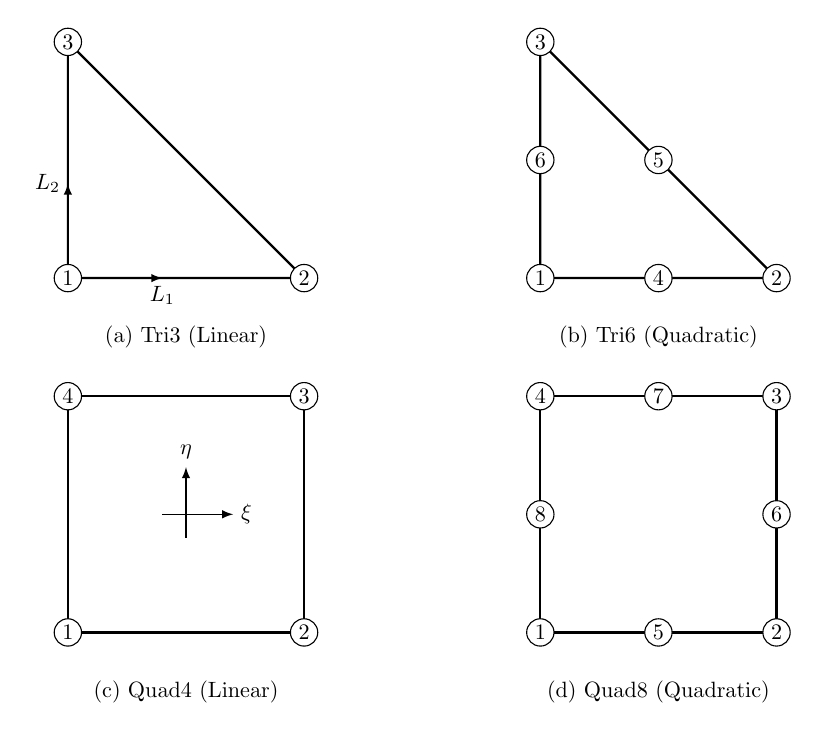
\begin{tikzpicture}[scale=1.5, every node/.style={scale=0.8}]
    \tikzstyle{node_style}=[circle, draw, fill=white, inner sep=1.5pt]
    \tikzstyle{elem_edge}=[thick]

    % --- (a) Tri3 ---
    \begin{scope}[shift={(0,3)}]
      \draw[elem_edge] (0,0) -- (2,0) -- (0,2) -- cycle;
      \draw[-latex] (0,0) -- (0.8,0) node[below]{$L_1$};
      \draw[-latex] (0,0) -- (0,0.8) node[left]{$L_2$};
      \node[node_style] at (0,0) {1};
      \node[node_style] at (2,0) {2};
      \node[node_style] at (0,2) {3};
      \node at (1, -0.5) {(a) Tri3 (Linear)};
    \end{scope}

    % --- (b) Tri6 ---
    \begin{scope}[shift={(4,3)}]
      \draw[elem_edge] (0,0) -- (2,0) -- (0,2) -- cycle;
      \node[node_style] at (0,0) {1};
      \node[node_style] at (2,0) {2};
      \node[node_style] at (0,2) {3};
      \node[node_style] at (1,0) {4};
      \node[node_style] at (1,1) {5};
      \node[node_style] at (0,1) {6};
      \node at (1, -0.5) {(b) Tri6 (Quadratic)};
    \end{scope}

    % --- (c) Quad4 ---
    \begin{scope}[shift={(0,0)}]
      \draw[elem_edge] (0,0) -- (2,0) -- (2,2) -- (0,2) -- cycle;
      \node[node_style] at (0,0) {1};
      \node[node_style] at (2,0) {2};
      \node[node_style] at (2,2) {3};
      \node[node_style] at (0,2) {4};
      \node at (1, -0.5) {(c) Quad4 (Linear)};
      % Axis
      \draw[-latex] (0.8,1) -- (1.4,1) node[right]{$\xi$};
      \draw[-latex] (1,0.8) -- (1,1.4) node[above]{$\eta$};
    \end{scope}

    % --- (d) Quad8 ---
    \begin{scope}[shift={(4,0)}]
      \draw[elem_edge] (0,0) -- (2,0) -- (2,2) -- (0,2) -- cycle;
      \node[node_style] at (0,0) {1};
      \node[node_style] at (2,0) {2};
      \node[node_style] at (2,2) {3};
      \node[node_style] at (0,2) {4};
      \node[node_style] at (1,0) {5};
      \node[node_style] at (2,1) {6};
      \node[node_style] at (1,2) {7};
      \node[node_style] at (0,1) {8};
      \node at (1, -0.5) {(d) Quad8 (Quadratic)};
    \end{scope}
  \end{tikzpicture}
  \caption{2次元アイソパラメトリック要素}\label{Fig:2D_Element_Library}
\end{figure}

\subsubsection{三角形要素群 (Triangular Elements)}
三角形要素では面積座標 $L_1, L_2, L_3$ を用いる.これらは $L_1+L_2+L_3=1$ を満たすため,独立変数は2つ(例: $L_1, L_2$)である.
一般の直交正規化座標 $(\xi, \eta)$ との対応は,通常 $\xi = L_1, \eta = L_2$ と定義される.

\begin{description}
  \item[一次三角形要素 (Tri3)]
        線形補間を行う最も基本的な要素である.
        \begin{equation}
          \psi_1 = L_1, \quad \psi_2 = L_2, \quad \psi_3 = L_3
        \end{equation}
  \item[二次三角形要素 (Tri6)]
        各辺の中点に節点を追加し,物理量の二次分布を表現可能とした要素である.
        \begin{align}
          \mbox{頂点節点:} & \quad \psi_1 = L_1(2L_1-1), \quad \psi_2 = L_2(2L_2-1), \quad \psi_3 = L_3(2L_3-1) \notag \\
          \mbox{中間節点:} & \quad \psi_4 = 4L_1L_2, \qquad~~ \psi_5 = 4L_2L_3, \qquad~~ \psi_6 = 4L_3L_1
        \end{align}
\end{description}

\subsubsection{四角形要素群 (Quadrilateral Elements)}
四角形要素では,正規化座標 $(\xi, \eta) \in [-1, 1] \times [-1, 1]$ を用いる.

\begin{description}
  \item[一次四角形要素 (Quad4)]
        双一次(Bilinear)補間を行う要素である.
        \begin{equation}
          \psi_i = \frac{1}{4}(1 + \xi_i \xi)(1 + \eta_i \eta) \quad (i=1,\dots,4)
        \end{equation}
        ここで $(\xi_i, \eta_i)$ は各節点の正規化座標である.
  \item[二次四角形要素 (Quad8)]
        各辺の中点に節点を追加したSerendipity族の二次要素である.中心節点を持たないため計算効率が良い.
        \begin{align}
          \mbox{隅節点 ($i=1\dots4$):} & \quad \psi_i = \frac{1}{4}(1 + \xi_i \xi)(1 + \eta_i \eta)(\xi_i \xi + \eta_i \eta - 1) \notag \\
          \mbox{中間節点 ($\xi_i=0$):}  & \quad \psi_i = \frac{1}{2}(1 - \xi^2)(1 + \eta_i \eta) \notag                                  \\
          \mbox{中間節点 ($\eta_i=0$):} & \quad \psi_i = \frac{1}{2}(1 + \xi_i \xi)(1 - \eta^2)
        \end{align}
\end{description}

\subsection{数値積分の統一的扱い}
剛性行列や質量行列の算出に必要な要素領域積分は,Gauss-Legendre積分公式を用いて次のように記述される.
\begin{equation}
  \label{Eq:Gauss-Legendre-2D}
  \int_{-1}^{+1}\int_{-1}^{+1} f\pab{\xi, \eta}\odif{\xi}\odif{\eta} \approx \sum_{i=1}^{N_\mathrm{sample}}\sum_{j=1}^{N_\mathrm{sample}}w_i w_j f\pab{\xi_i, \eta_j}
\end{equation}
ただし,$N_\mathrm{sample}$は各軸方向のサンプル点数,$w_i$は重み,$\xi_i$,$\eta_i$はガウス積分点である.

\eqref{Eq:Gauss-Legendre-2D}を用いたときの積分の概念図を示す.このとき,サンプル点は2点とする.

\begin{figure}[H]
  \centering
  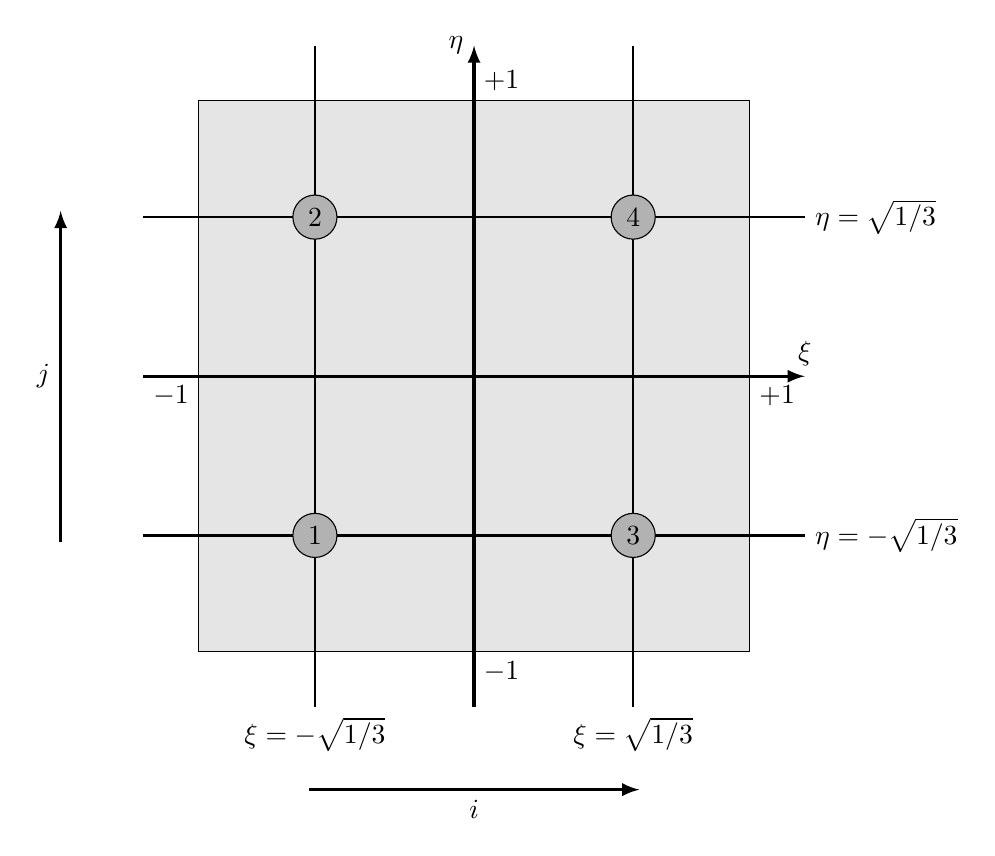
\begin{tikzpicture}[scale=3.5]
    \coordinate (p1) at (-1,-1);
    \coordinate (p2) at (1,-1);
    \coordinate (p3) at (1,1);
    \coordinate (p4) at (-1,1);
    \coordinate (S1) at (-0.57735,-0.57735);
    \coordinate (S2) at (-0.57735, 0.57735);
    \coordinate (S3) at ( 0.57735,-0.57735);
    \coordinate (S4) at ( 0.57735, 0.57735);

    % 背景の領域(元々薄いグレーなのでそのまま)
    \draw[fill=black!10!white] (p1)--node[midway, below right]{$-1$}(p2)--node[midway, below right]{$+1$}(p3)--node[midway, above right]{$+1$}(p4)--cycle node[midway, below left]{$-1$};
    %axis
    \draw[-{latex}, line width=0.4mm] (-1.2,0) -- (1.2,0) node[above]{$\xi$};
    \draw[-{latex}, line width=0.4mm] (0,-1.2) -- (0,1.2) node[left]{$\eta$};

    \draw[-{latex}, line width=0.4mm] (-0.6,-1.5) --node[midway, below]{$i$} (0.6,-1.5);
    \draw[-{latex}, line width=0.4mm] (-1.5,-0.6) --node[midway, left]{$j$} (-1.5,0.6);

    \draw[-, line width=0.3mm] (-1.2, 0.57735) -- (1.2, 0.57735) node[right]{$\eta= \sqrt{1/3}$};
    \draw[-, line width=0.3mm] (-1.2,-0.57735) -- (1.2,-0.57735) node[right]{$\eta=-\sqrt{1/3}$};
    \draw[-, line width=0.3mm] (-0.57735,-1.2) node[below]{$\xi=-\sqrt{1/3}$} -- (-0.57735,1.2);
    \draw[-, line width=0.3mm] ( 0.57735,-1.2) node[below]{$\xi= \sqrt{1/3}$} -- ( 0.57735,1.2);

    % サンプル点の円(ピンクからグレーに変更)
    \foreach \i in {1,2,3,4} {
        \draw[fill=gray!60] (S\i) node {\i} circle[radius=0.08];
      }
  \end{tikzpicture}
  \caption{Gauss-Legendre積分のサンプル点を2点とした場合の概念図}
\end{figure}

サンプル点数に応じた重みとガウス積分点を\cref{Table:Gauss-Legendre-PointsAndWeights}に示す.なお,重み $w_i$ は1次元積分における値であり,2次元積分ではその積 $w_i w_j$ が用いられる.
\begin{longtable}{ccc}
  \caption{Gauss-Legendre積分のサンプル点数とガウス積分点,および重み}\label{Table:Gauss-Legendre-PointsAndWeights}                        \\
  \hline
  点数:$N_\mathrm{sample}$ & 座標:$\xi_i$,$\eta_i$                                      & 重み:$w_i$                       \\
  \hline
  $1$                    & $0$                                                      & $2$                            \\
  \hline
                         &                                                          &                                \\[-6mm]
  $2$                    & $\pm\sqrt{\dfrac{1}{3}}$                                 & $1$                            \\[7mm]
  \hline
                         &                                                          &                                \\[-6mm]
  $3$                    & $0$                                                      & $\dfrac{8}{9}$                 \\[7mm]
                         & $\pm\sqrt{\dfrac{3}{5}}$                                 & $\dfrac{5}{9}$                 \\[7mm]
  \hline
                         &                                                          &                                \\[-6mm]
  $4$                    & $\pm\sqrt{\dfrac{3}{7}-\dfrac{2}{7}\sqrt{\dfrac{6}{5}}}$ & $\dfrac{18+\sqrt{30}}{36}$     \\[7mm]
                         & $\pm\sqrt{\dfrac{3}{7}+\dfrac{2}{7}\sqrt{\dfrac{6}{5}}}$ & $\dfrac{18-\sqrt{30}}{36}$     \\[7mm]
  \hline
                         &                                                          &                                \\[-6mm]
  $5$                    & $0$                                                      & $\dfrac{128}{225}$             \\[7mm]
                         & $\pm\dfrac{1}{3}\sqrt{5-2\sqrt{\dfrac{10}{7}}}$          & $\dfrac{322+13\sqrt{70}}{900}$ \\[7mm]
                         & $\pm\dfrac{1}{3}\sqrt{5+2\sqrt{\dfrac{10}{7}}}$          & $\dfrac{322-13\sqrt{70}}{900}$ \\[7mm]
  \hline
\end{longtable}

有限要素法における数値積分では,被積分関数(形状関数の導関数やヤコビアンの積)の次数に応じて適切な積分点数を選択する必要がある.$N_\mathrm{sample}$ 点のGauss-Legendre積分は $2N_\mathrm{sample}-1$ 次以下の多項式を厳密に積分可能である.剛性行列の評価には通常,フル積分(Full Integration)が推奨されるが,計算効率の向上やロッキング現象の回避を目的として,意図的に積分点数を減らす低減積分(Reduced Integration)が用いられる場合もある.
ここで,要素タイプごとの標準的な積分規則を\cref{Table:Integration_Rules}に示す.
\begin{table}[H]
  \centering
  \caption{各要素タイプにおける標準的な数値積分則}
  \label{Table:Integration_Rules}
  \begin{tabular}{lcccc} \toprule
    要素    & 座標系        & 積分点数              & 積分次数     & 備考     \\ \midrule
    Tri3  & 面積座標       & 1点                & $O(h)$   & 重心積分   \\
    Tri6  & 面積座標       & 3点                & $O(h^2)$ & 辺の中点など \\
    Quad4 & $\xi-\eta$ & $2 \times 2 = 4$点 & $O(h^2)$ & フル積分   \\
    Quad8 & $\xi-\eta$ & $3 \times 3 = 9$点 & $O(h^3)$ & フル積分   \\ \bottomrule
  \end{tabular}
\end{table}

\FloatBarrier
